\selectlanguage{english}
\begin{abstract}
    \noindent A \emph{Számítógépes szimulációk} című laboratúrium első alkalmával az egyszerű, 1 dimenziós harmonikus oszcillátor mozgásegyenletének numerikus megoldását járjuk körül, mely a félévi tárgy bevezetőjeként szolgál. A szimuláció forráskódja C++ nyelven, az adatok elemzése és az ábrák pedig egy Jupyter Notebook-ban futó Python 3 kernel alatt készültek. A beadandó első célja a forráskóddal történő ismerkedés, valamint a paraméterek változtatásával történő különböző kezdőfeltételek beállítása és a szimuláció futtatása volt. Ezt követően az ebből kapott különböző kimenetek, megadott szempontok alapján történő elemzése volt a feladatunk. \\
\end{abstract}
\selectlanguage{magyar}

\begin{multicols}{2}
\section{Bevezetés és elmélet} \label{sec:1}
A Számítógépes szimulációk laboratórium első feladata során az egyszerű, 1-dimenziós harmonikus oszcillátor mozgását vizsgáltuk. Fizikai modelljének leírása és a szimuláció forráskódja már előzetesen a rendelkezésünkre állt a tárgy honlapján\cite{szamszin}. \\
Az 1D harmonikus oszcillátort az alábbi mozgásegyenlettel írhatjuk le:

\begin{equation} \label{eq:1.1}
    m * \ddot{x} \left( t \right)  = - m * \omega^{2} * x \left( t \right)
\end{equation}
Ennek a differenciálegyenletnek az analitikus megoldását egy megfelelő Ansatz segítségével kaphatjuk meg a legkönnyebben. Az egyenlet megoldása a következő lesz:

\begin{equation} \label{eq:1.2}
    x \left( t \right)  = x_{0} * \cos(\omega t) + \frac{v_{0}}{\omega} * \sin(\omega t)
\end{equation}
A numerikus megoldáshoz a mozgásegyenlet alábbi formáját használjuk fel:

\begin{equation} \label{eq:1.3}
    \frac{d^{2} x \left( t \right) }{d t^{2}} = - \omega^{2} * x \left( t \right) 
\end{equation}
Ugyanis ezt felbonthatjuk a következő két, elsőrendő, csatolt egyenletre:

\begin{equation} \label{eq:1.4}
    \frac{dx \left( t \right)}{dt} = v \left( t \right) 
\end{equation}

\begin{equation} \label{eq:1.5}
    \frac{dv \left( t \right)}{dt} = - \omega^{2} * x \left( t \right) = a \left( t \right)
\end{equation}
Ez az egyenletrendszer analitikusan is könnyen megoldható, azonban a gyakorlás kedvéért numerikus megoldáshoz folyamodunk.

\section{Feladatok} \label{sec:2}
Az első szimuláció során négy darab feladatot volt szükséges teljesíteni a rendelkezésre álló forráskód fordítása után. \\
Az első a harmonikus oszcillátor kitérés-idő diagramjának felvétele tetszőlegesen hosszú időtartamra. \\
A második feladatban az oszcillátor kitérés-sebesség diagramját kell vizsgálnunk hosszú időtartamra. Itt elemeznünk és diszkutálnunk is kell a kapott eredményt, hogy miben tér el a várt képtől. \\
A harmadik feladat az Euler-Cromer és a szimpla Euler differenciálegyenlet megoldási módszerek összehasonlítása az energiamegmaradás szempontjából. A fő kérdés, hogy melyiknél és hogyan marad, vagy nem marad meg az energia? \\
A negyedik feladat során a szimuláció futásidejét kell tesztelnünk és megvizsgálnunk a megoldási módszerekben használt lépésszám függvényében.

\section{Megvalósítás} \label{sec:3}
A szimuláció forráskódja C++ nyelven készült és az Euler-Cromer megoldási módszert alkalmazza, mely az Euler módszer apró bővítéssel ellátott verziója. Az Euler módszer lényege a következő, a fent ismertetett egyenleteken keresztül bemutatva\cite{csabaidiff}:

\begin{equation}
    v \left(t + \Delta t \right) = v \left( t \right) - \omega^{2} * x \left( t \right) * \Delta t
\end{equation}

\begin{equation}
    x \left(t + \Delta t \right) = x \left( t \right) + v \left( t \right) * \Delta t
\end{equation}

\begin{equation}
    t \to t + \Delta t
\end{equation}
Ennek módosított variációja a már említett Euler-Cromer módszer, ahol a második lépésben nem a $t$, hanem a $t + \Delta t$ helyen levő értékkel történik a kiértékelés. A módszer kontraintuitívnak tűnhet az alábbi módon:

\begin{equation}
    v \left(t + \Delta t \right) = v \left( t \right) - \omega^{2} * x \left( t \right) * \Delta t
\end{equation}

\begin{equation}
    x \left(t + \Delta t \right) = x \left( t \right) + v \left( t + \Delta t \right) * \Delta t
\end{equation}

\begin{equation}
    t \to t + \Delta t
\end{equation}
Mindkét esetben az $x \left( t = 0 \right)$ és a $v \left( t = 0 \right)$ értékekkel inicializáljuk a szimulációnkat, majd addig futtatjuk, míg a $t$ érték el nem ér egy tetszőleges $t_{max}$ felső korlátot. $\Delta t$ a szimuláció lépésközét jelöli, amit szintén mi választunk meg. \\
Várakozásaink szerint az utóbbi módszer előnye, hogy szinte megtartja az energiát, míg az első nem\cite{cromer}. Ez persze egyéb módszerek segítségével még tovább javítható, azonban ennek a tárgyalásába most nem megyünk bele\cite{Iserles-2003}. Az Euler és Euler-Cromer módszerek energiaviszonyainak vizsgálata majd a harmadik részfeladatban fog megtörténni.

\subsection{A rendelkezésre álló kód modosításai}
Az eredeti forráskódon több változtatást kellett végrehajtani, hogy a kiszabott feladatokat meg lehessen vele oldani. Első lépésben az eredeti \code{sho.cpp} file-ból létrehoztam egy \code{sho\_e.cpp} és egy \code{sho\_ec.cpp} varióciót. Az utóbbi az eredeti Euler-Cromer formulával megadott forráskód volt, míg az elsőben - az eredeti változtatásával - az Euler módszert implementáltam. A forráskódokat egy-egy segéd batch file segítségével fordítottam le, abban clang fordítót használva, mely kimeneti binárisa így egy \code{sho\_e.exe} és egy \code{sho\_ec.exe} lett. Az \cite{szamszin} linken elérhető forráskód ellenben egyéb pontokban is apró módosításokra szorult. \\
A második alapvető módosítás eredménye az, hogy a szimulációk végleges kimenetként egy \emph{sho.dat} nevű file-t generálnak, ami az adatokat az \ref{tab1}. táblázatnak megfelelő elrendezésben tartalmazza.

\begin{center}
\begin{tabular}{c|c|c|c|c}
$t$ & $x \left( t \right)$ & $v \left( t \right)$ & $E \left( t \right)$ & $T_{fut} \left( t \right)$ \\
\hline \hline
$0$ & $x \left( 0 \right)$ & $v \left( 0 \right)$  & $E \left( 0 \right)$ & $T_{fut} \left( 0 \right)$ \\
\hline
$\Delta t$ & $x \left( \Delta t \right)$ & $v \left( \Delta t \right)$ & $E \left( \Delta t \right)$ & $T_{fut} \left( \Delta t \right)$ \\
\hline
$2 \Delta t$ & $x \left( 2 \Delta t \right)$ & $v \left( 2 \Delta t \right)$ & $E \left( 2 \Delta t \right)$ & $T_{fut} \left( 2 \Delta t \right)$ \\
\hline
\vdots & \vdots & \vdots & \vdots & \vdots \\
\hline
$t_{max}$ & $x \left( \Delta t_{max} \right)$ & $v \left( \Delta t_{max} \right)$ & $E \left( \Delta t_{max} \right)$ &$T_{fut}$ \\
\hline
\end{tabular}
\end{center}
\captionof{table}{Az output \code{.dat} file-ok szerkezete}\label{tab1}
\hfill \break \hfill \break
\noindent A következő változtatás motivációja a programok könnyebb futtathatóságának célja volt. Ezt megoldandó, a programok a szimulációs paramétereket terminálban megadott argumentumok formájában várják (ebből 5 darab van), amiket végül egy Juypter Notebook cella futtat az \code{os} package segítségével az alábbi módon, ahol az XX a tetszőlegesen választható \code{e}, vagy \code{ec} végződést helyettesíti:
\begin{center}
    \code{os.system('sho\_XX.exe\ ' + str(omega) +\ ' '\ + str(x\_0) +\ ' '\ +  str(v\_0) +\ ' '\ + str(t) +\ ' '\ + str(dt))}
\end{center}
Ahol $\omega$ (omega) a rezgés körfrekvenciáját, $x_{0}$ (x\_0) és $v_{0}$ (v\_0) rendre a kezdő kitérés és sebesség nagyságát, $t$ a szimulálandó periódusok számát, $dt$ pedig a periódusonkénti lépésközt jelenti. \\
Az utolsó módosítás a negyedik feladatban szereplő időméréshez szükséges módosításokat foglalja magába. Ezt a C++ chrono library mikroszekundomos pontosságú időmérési módszerét felhasználva oldottam meg. \\
A véglegesített forráskód és az azt futtató Notebook elérhető GitHub-on\cite{github}.

\section{Kiértékelés}
Az adatok elemzését egy Jupyter Notebook Python 3 kernelében végeztem el. Ez a notebook szintén elérhető a szimuláció GitHub repository-jában\cite{github}.

\subsection{Kitérés-idő diagram}
Az első feladatban a harmonikus oszcillátor kitérésének és sebességének viselkedését figyeltük az idő függvényében. A szimuláció kezdőfeltételei a \ref{tab2}. ábrán olvashatóak.
\begin{center}
\begin{tabular}{c|c}
Szim. paraméter & Érték \\
\hline \hline
$\omega$ & $15$ \\
\hline
$x_{0}$ & $0$ \\
\hline
$v_{0}$ & $5$ \\
\hline
$t$ & $10$ \\
\hline
$dt$ & $100$ \\
\hline
\end{tabular}
\end{center}
\captionof{table}{A szimuláció első feladatának kezdőfeltételei}\label{tab2}
\hfill \break \hfill \break
{\centering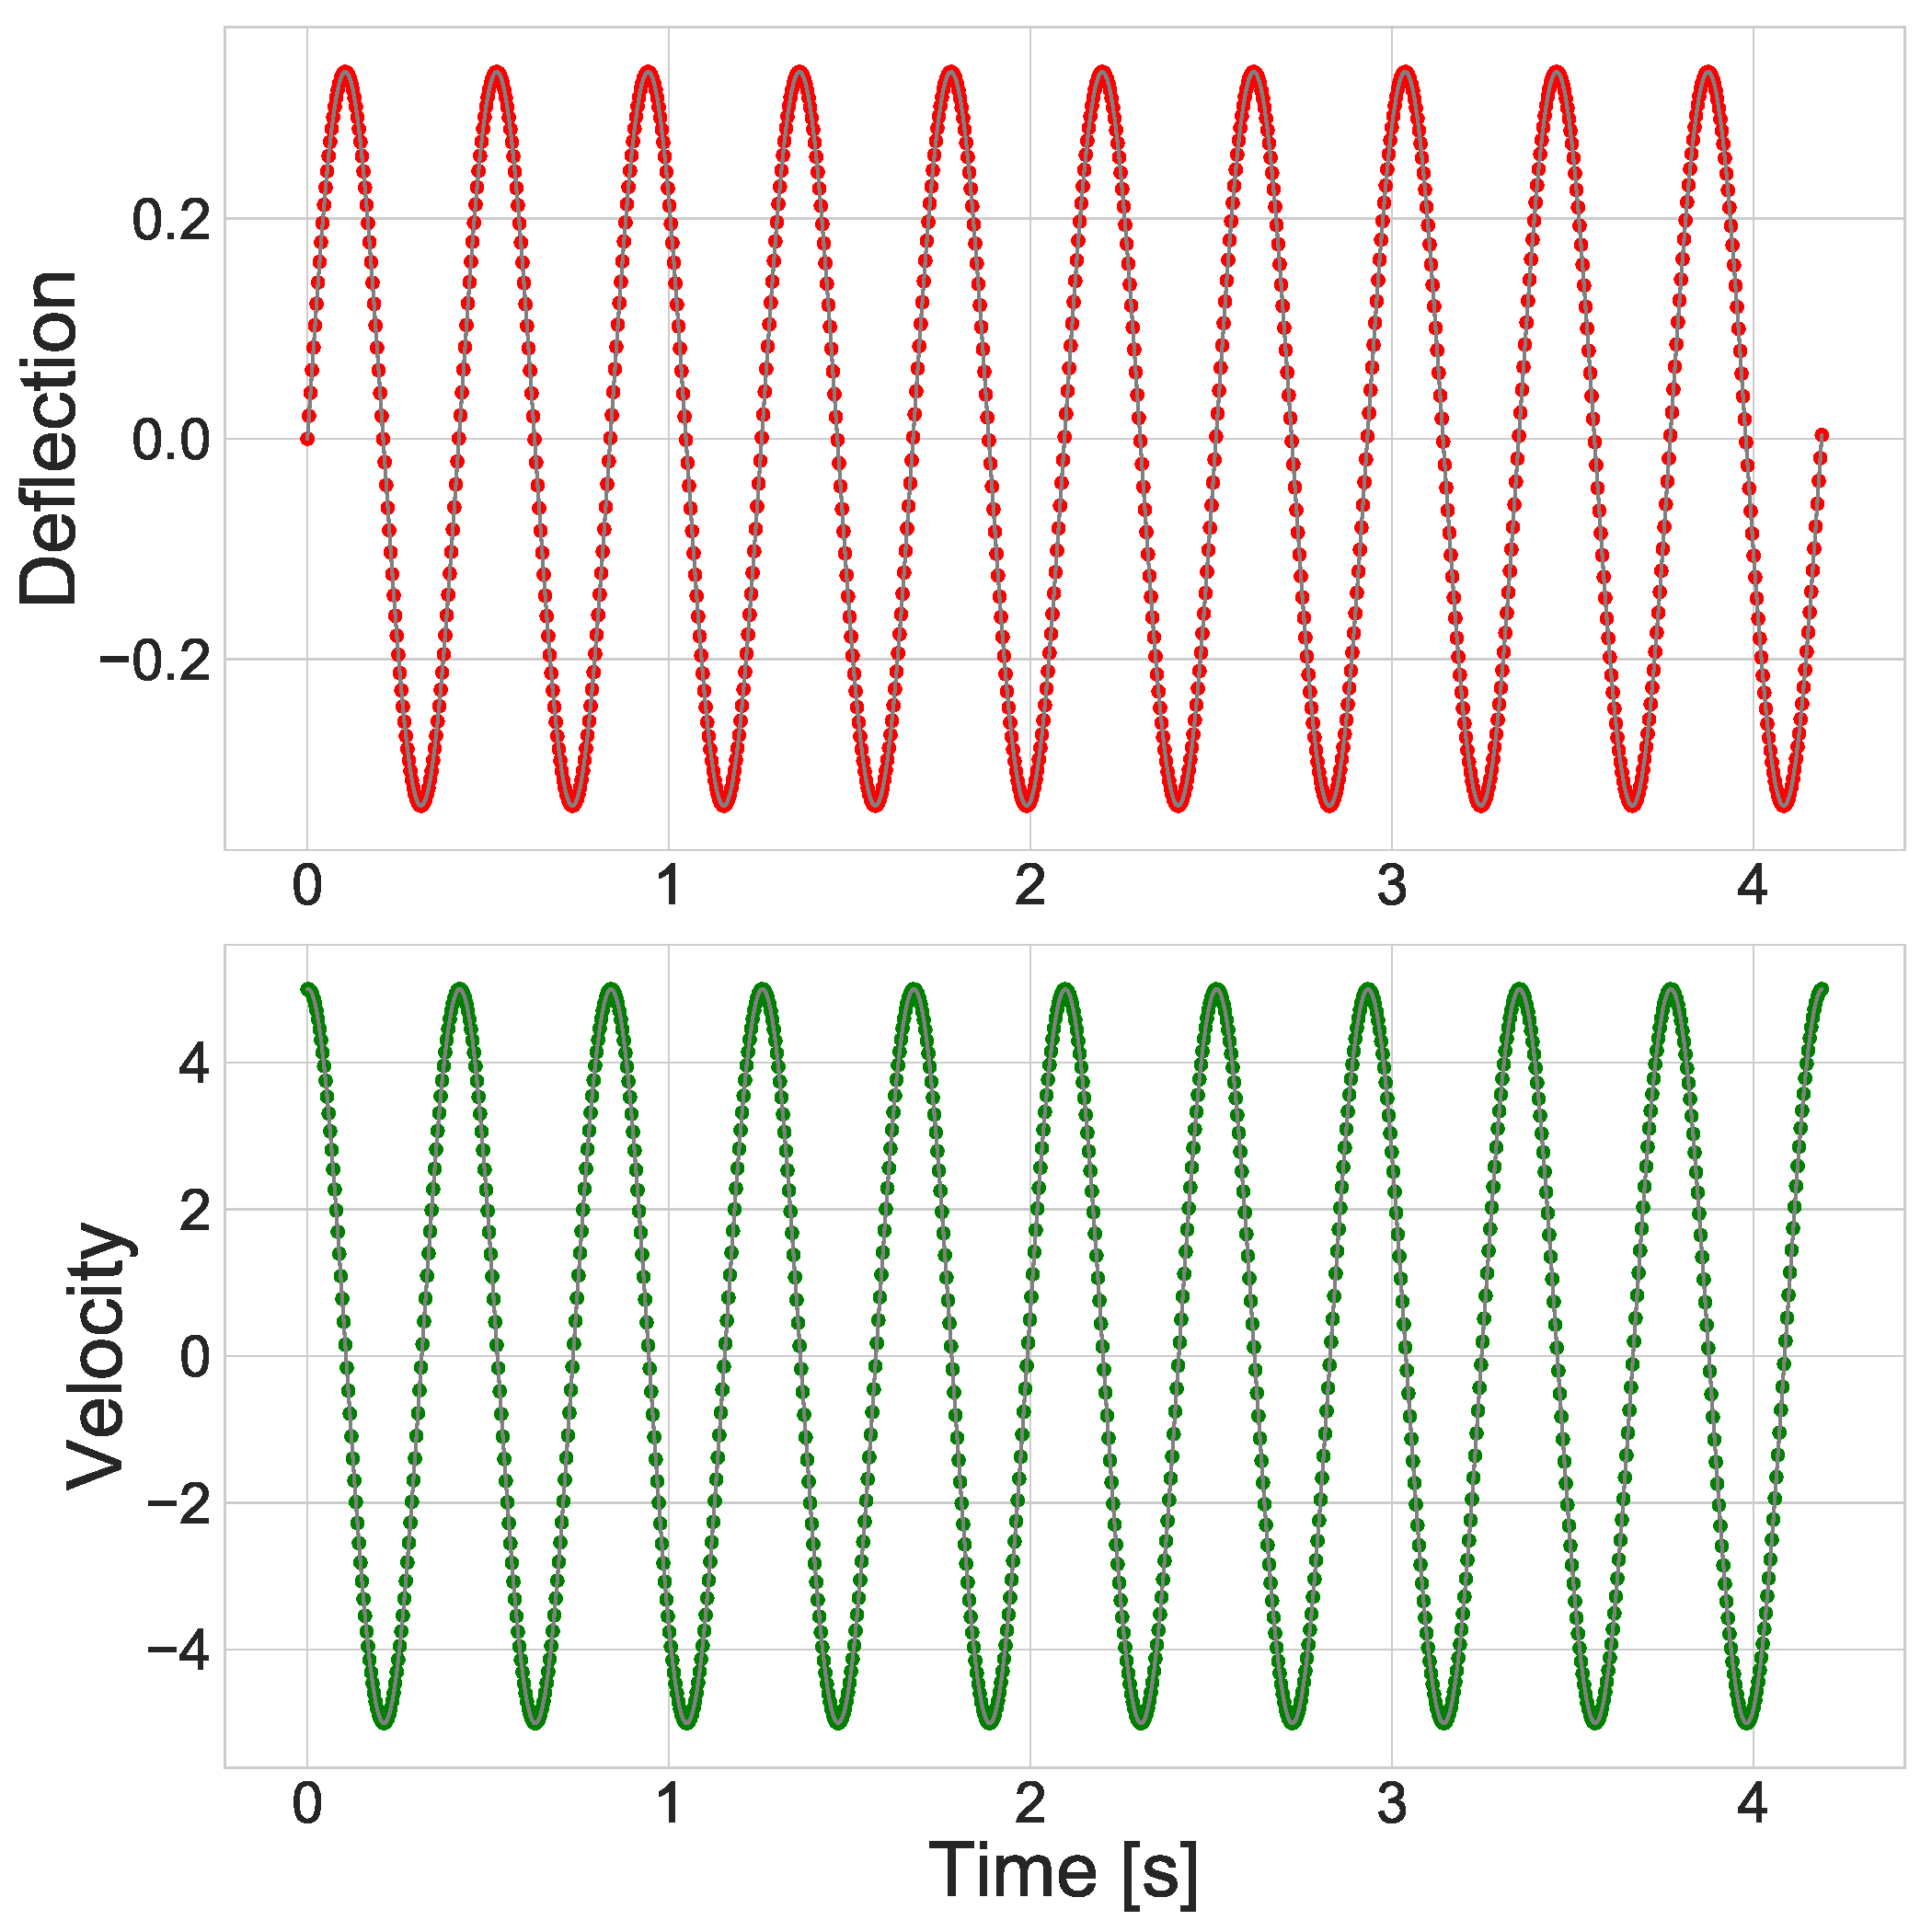
\includegraphics[width=.5\textwidth]{time_def_vel_eulercromer.pdf}}
\captionof{figure}{Euler-Cromer módszer\\Fent: Idő - Kitérés grafikon\\Alul: Idő - Sebesség grafikon}\label{fig1}
\hfill \break \hfill \break
A szimuláció során kapott adatok az első feladatnak megfelelően az \ref{fig1}. ábrán láthatóak. Ez a mélyebb megértés céljából egy sebesség-idő grafikonnal is ki lett bővítve. A kapott kép alapján az elméletből elvártakat kaptuk vissza. Az oszcillátor sebessége zéró kitérésnél a legnagyobb, maximális kitérésnél $0$, majd pedig előjelet vált.

\subsection{Kitérés-sebesség diagram}
A második feladatban a szimulációt nagyon hosszú idejű futtatásra kellett vizsgálni. Az elméleti ismertetőben már szó volt róla, hogy az Euler-Cromer módszer a natív Euler módszernél jobban, teljesen megőrzi az energiát. Az elmélet szerint azt várnánk, hogy bármilyen hosszú idejű futtatásra is, a kitérés-sebesség diagram egy ellipszist adna eredményül, mely ugyanabba a pontba tér vissza egész számú periódusra vizsgálva. Mivel azonban a differenciálegyenlet ezen megoldási módszere sem teljesen tökéletes, így ez hosszabb idejű futtatásra már nem lesz igaz. Míg rövid idejű futás esetén ($\sim 10$ periódus) nem lesz számottevő eltérés, addig nagyobb számú periódus ($\sim 1000$) esetén a kitérés-idő diagram nem ugyanabba a pontba fog visszatérni. A két eset összehasnolítása a \ref{fig2}. ábrán látható, a hozzá felhasznált szimulációs paraméterek pedig a \ref{tab3}. táblázatban találhatóak.

\begin{center}
\begin{tabular}{c|c|c}
Szim. paraméter & Rövid futás & Hosszú futás \\
\hline \hline
$\omega$ & $15$ & $15$ \\
\hline
$x_{0}$ & $0$ & $0$ \\
\hline
$v_{0}$ & $5$ & $5$ \\
\hline
$t$ & $10$ & $1000$ \\
\hline
$dt$ & $100$ & $100$ \\
\hline
\end{tabular}
\end{center}
\captionof{table}{A szimuláció második feladatának kezdőfeltételei}\label{tab3}
\hfill \break \hfill \break
{\centering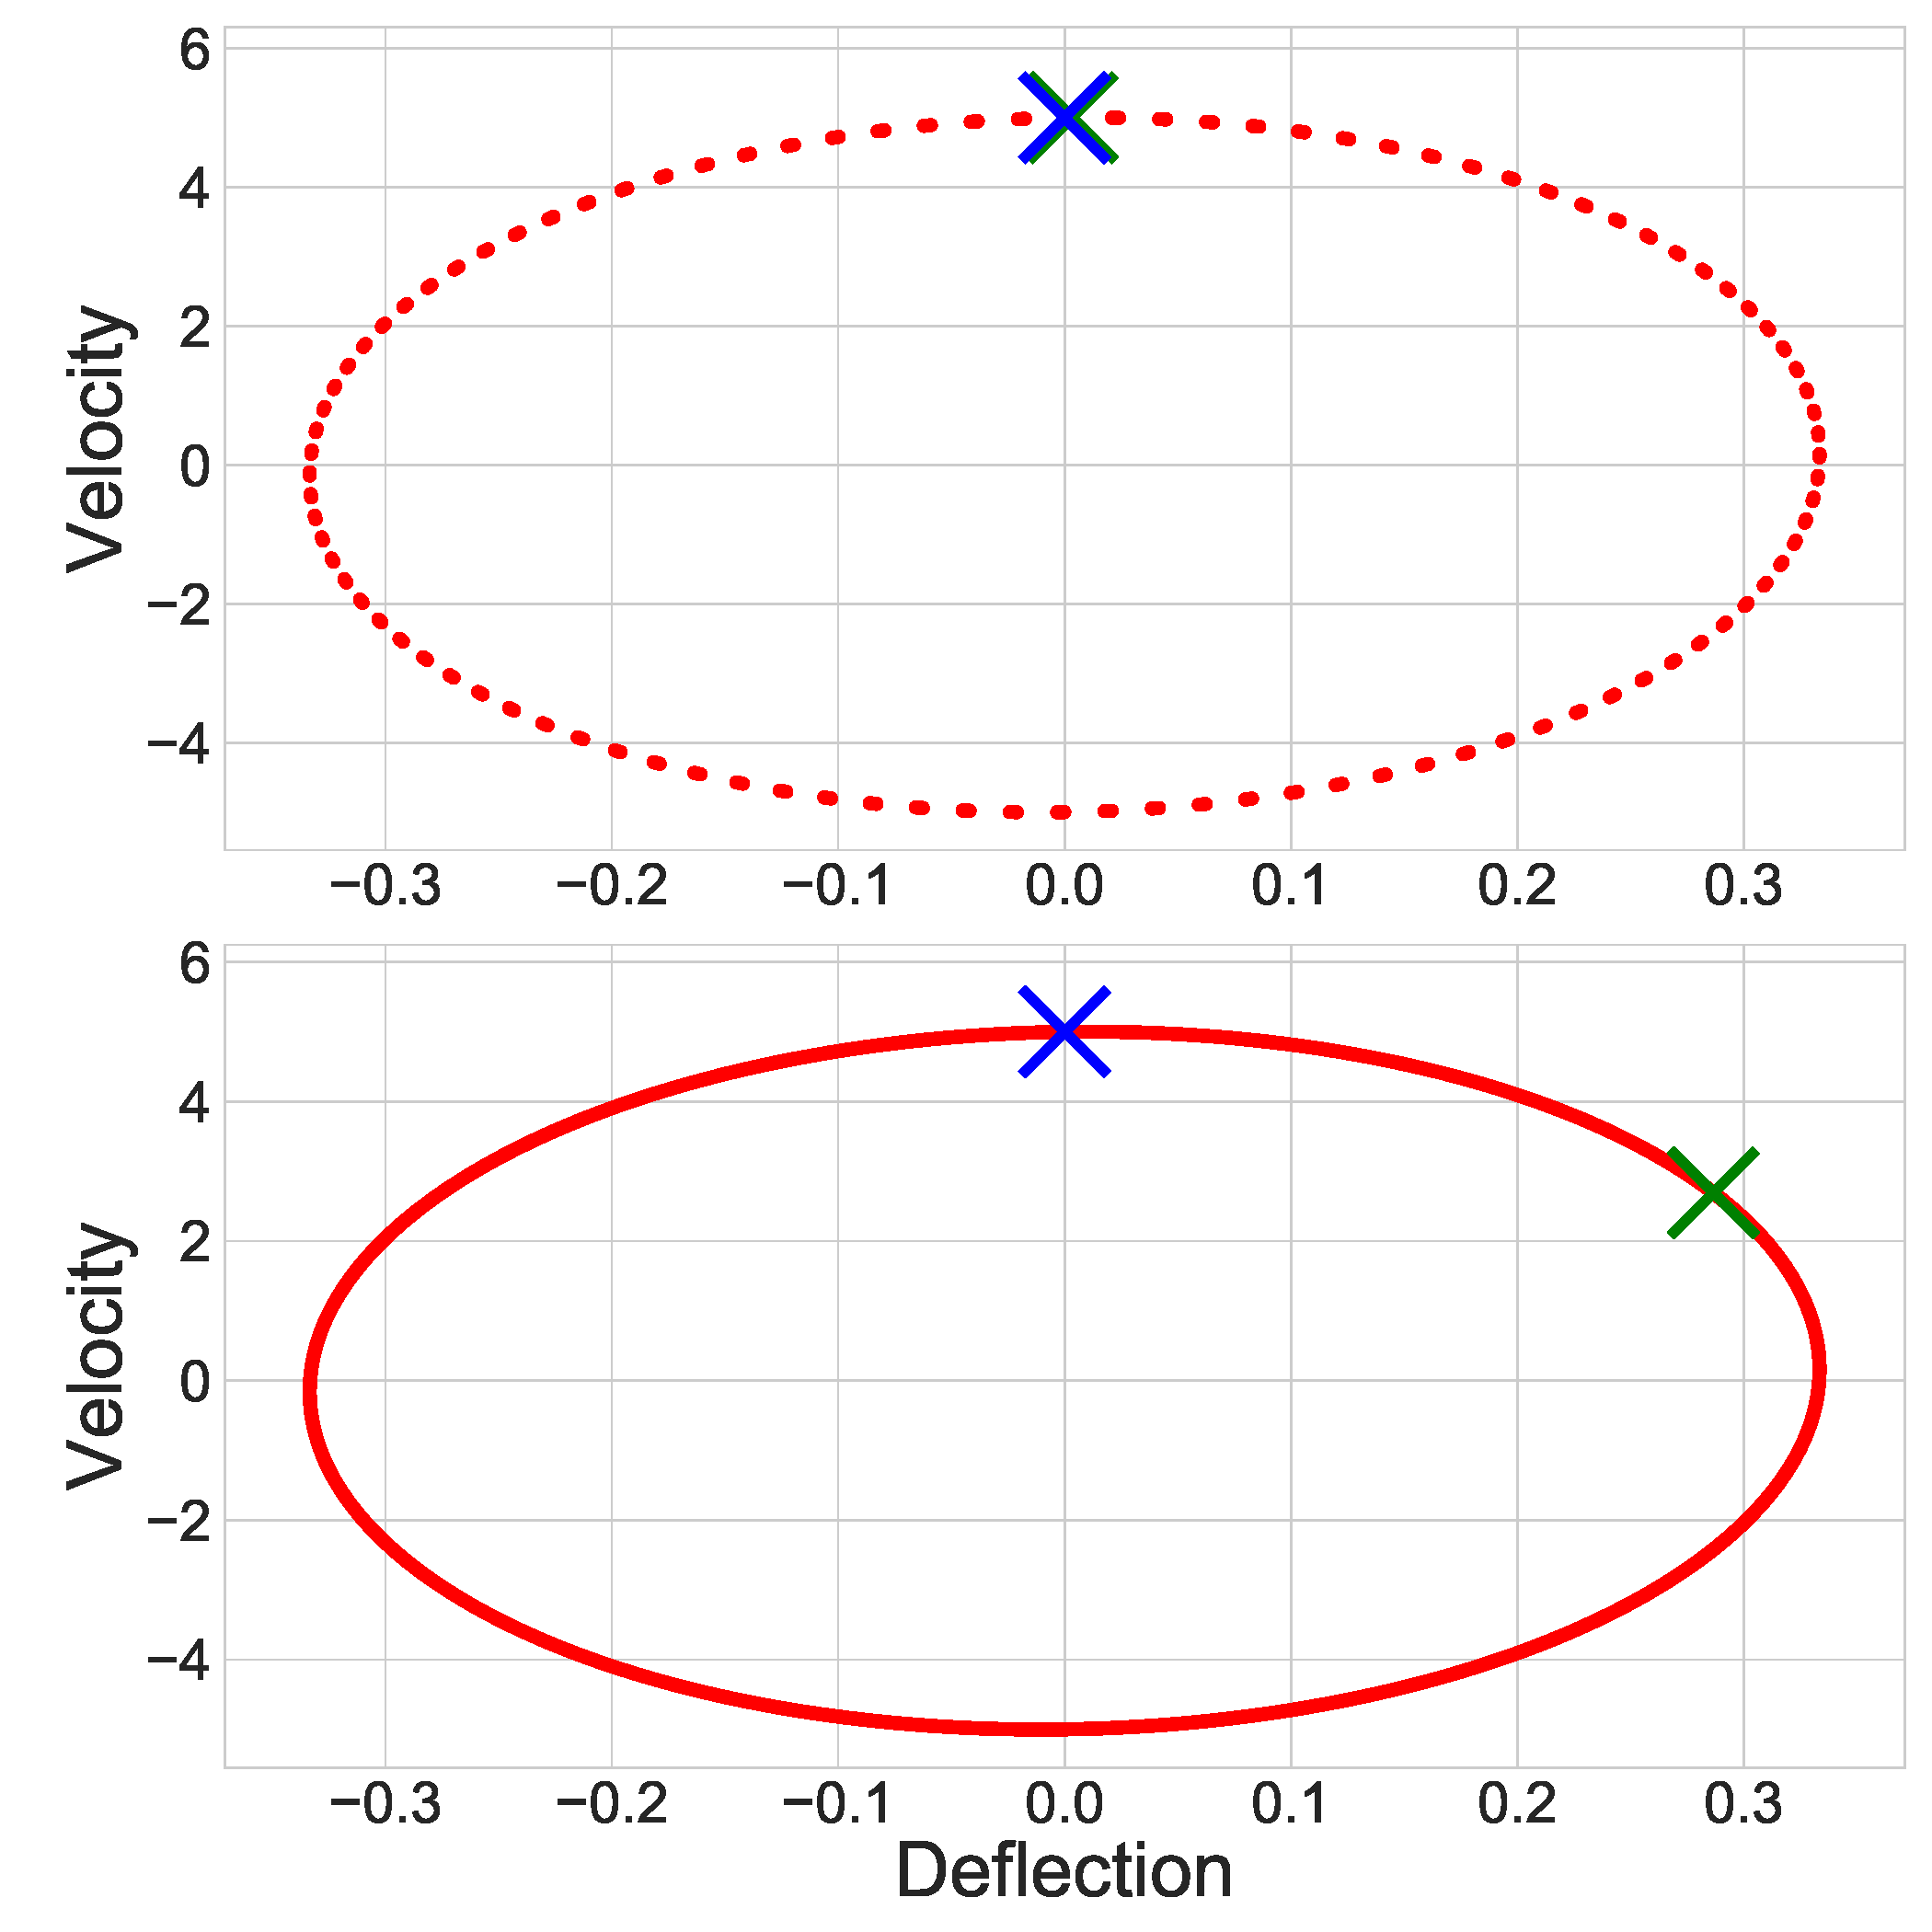
\includegraphics[width=.5\textwidth]{def_vel_long_eulercromer.pdf}}
\captionof{figure}{Euler-Cromer rövid és hosszú futás\\Fent: Kitérés - Sebesség grafikon rövid futásidő esetén\\Alul: Kitérés - Sebesség grafikon hosszú futásidő esetén}\label{fig2}
\hfill \break \hfill \break
A \ref{fig2}. ábrán a \textcolor{blue}{kék $X$} a szimuláció kezdőpontját míg a \textcolor{ForestGreen}{zöld $X$} a végpontját jelenti. Míg az első ábrán teljesen fedik egymást, addig a másodikon tisztán látszik, hogy a periódusok nagy mértékben \q{elcsúsznak}.

\subsection{Energiamegmaradás}
A harmadik feladatban a natív Euler és az Euler-Cromer differenciálegyenlet megoldási módszereket kellett összehasonlítanunk az energiamegmaradás szempontjából. Ez szorosan kapcsolódik az előbbi feladathoz, ugyanis itt is szintén a szimuláció hosszabb távú pontossága a kérdés. \\
Hogy összehasonlíthassuk a két módszert, az eredeti - már módosított - file-ról másolatot készítettem és az Euler-Cromer módszer módosításával abban implementáltam a natív Euler módszert. Ezt a két programot szimultán futtattam, azonos, az \ref{tab1}. táblázatban szereplőekkel megegyező paraméterekkel, amiket újfent egy Jupyter Notebook-ban futó Python 3 kernel segítségével hasonlítottam össze. \\
Az Euler módszer esetén az energia nem marad meg, folyamatosan növekszik az idő előrehaladtával. Ez abból adódik, hogy az oszcillátor kitérése és sebessége a nem teljesen optimális léptetés miatt szintén folyamatosan növekszik, az energia pedig ismert módon ezek által határozódik meg. A \ref{fig3}. ábrán az így futtatott program idő-energia, kitérés-energia és sebesség-energia grafikonjait láthatjuk. A szimuláció kezdőfeltételei megegyeznek az \ref{tab2}. Az \ref{fig4}. ábrán érdekességképpen az Euler módszerrel kapott kitérés-sebesség grafikont ábrázoljuk. A \ref{fig2}. ábrához hasonló jelölés segítségével látható, hogy a várt ellipszis helyett egy kifelé terjedő spirált kapunk. Ezzel összehasonlítandó, az Euler-Cromer módszer segítségével lefuttatott szimuláció energiaviszonyairól a \ref{fig5}. ábráról tájékozódhatunk.
\hfill \break \hfill \break
{\centering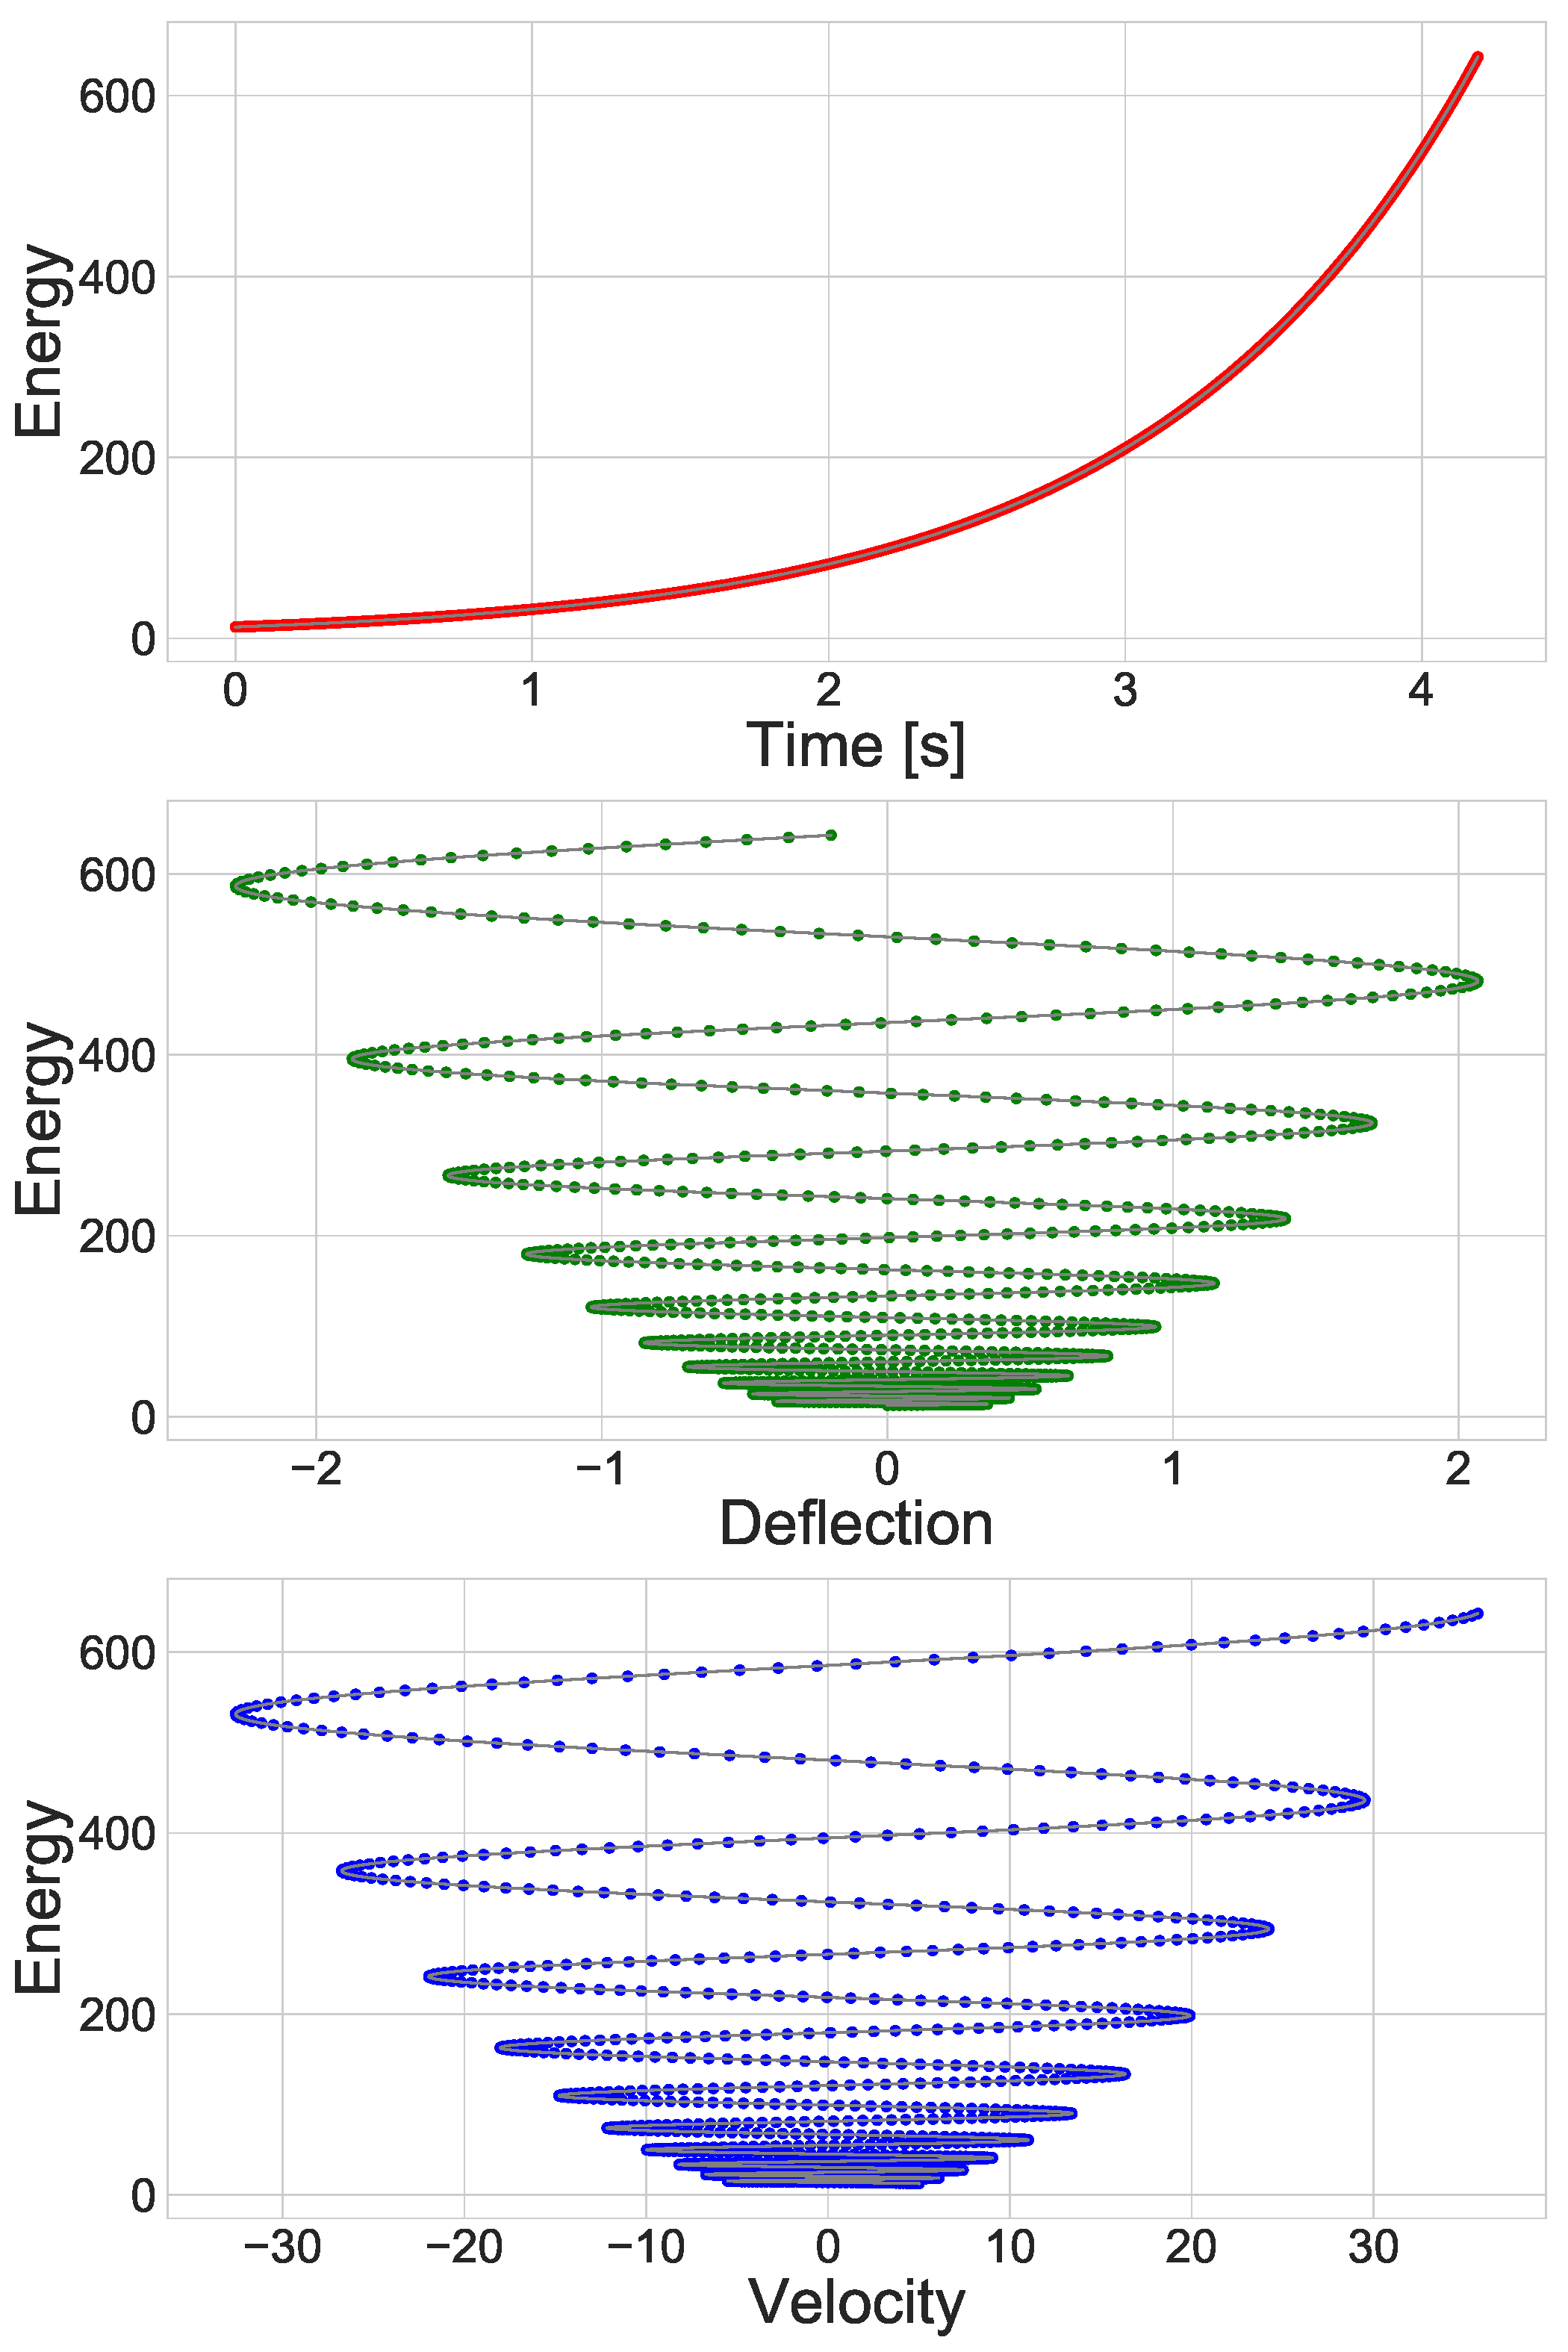
\includegraphics[width=.5\textwidth]{energy_euler.pdf}}
\captionof{figure}{Euler módszer\\Fent: Idő - Energia\\Középen: Kitérés - Energia\\Alul: Sebesség - Energia}\label{fig3}
\hfill \break \hfill \break
{\centering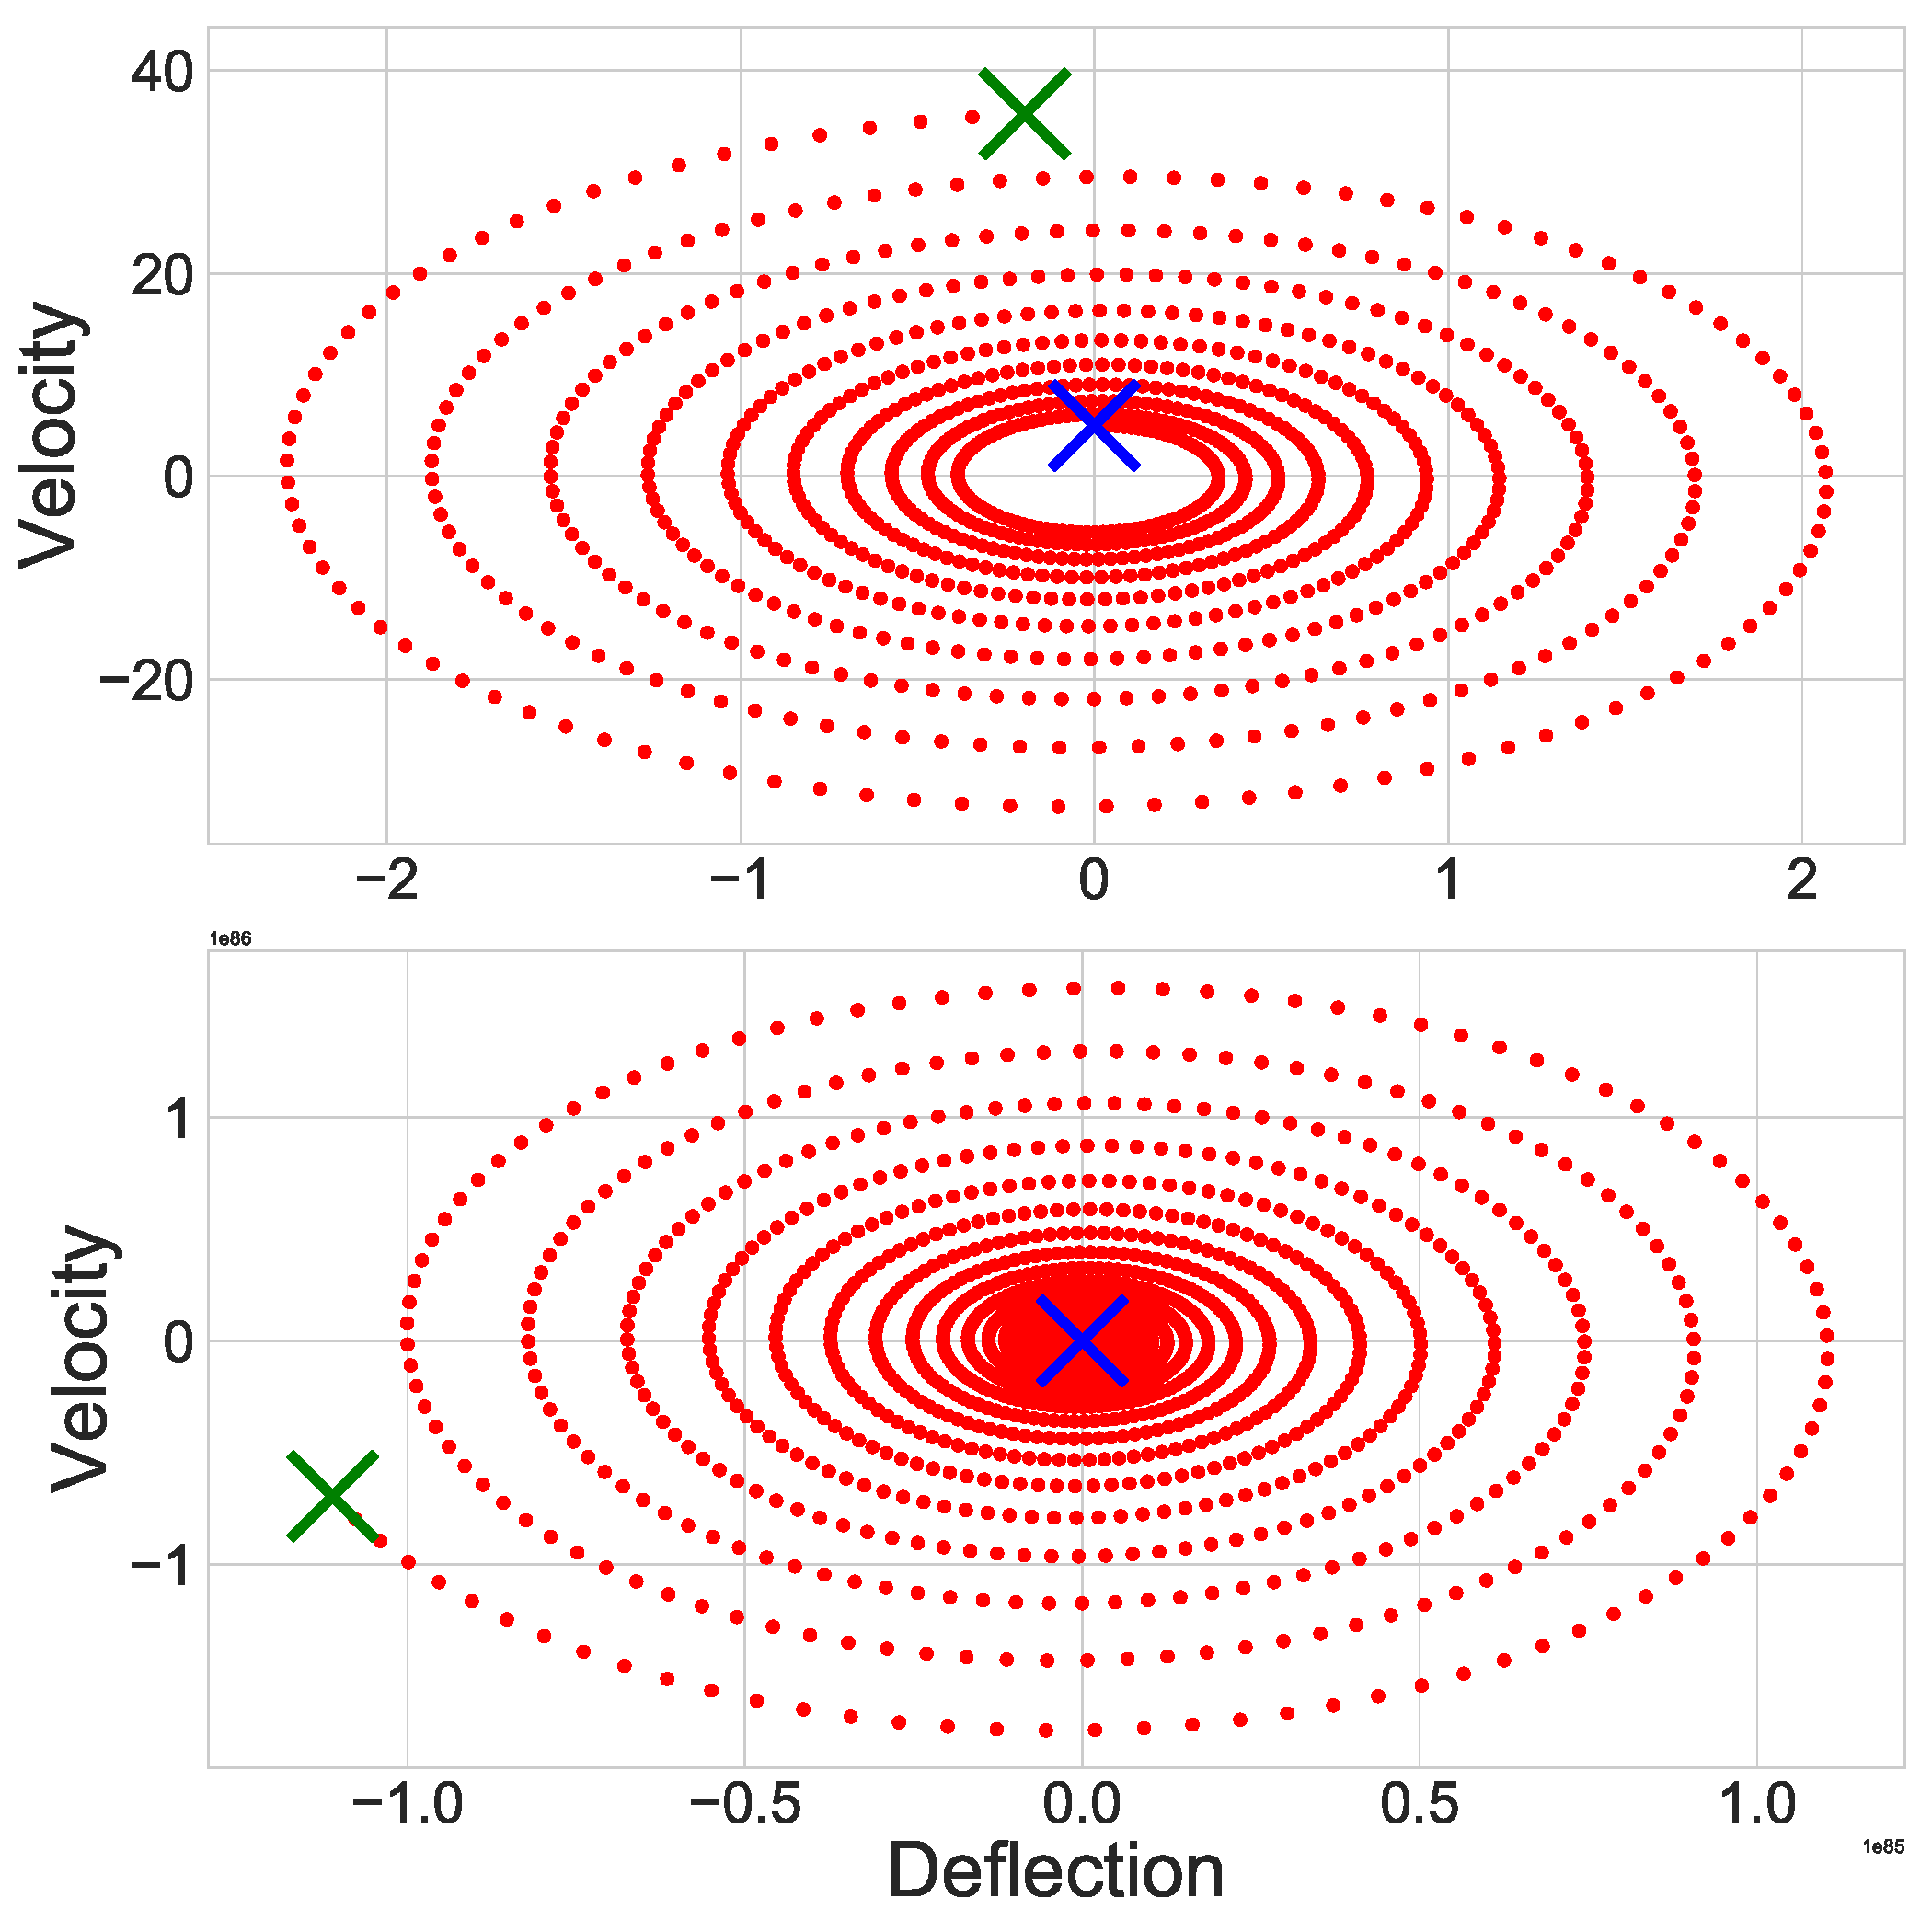
\includegraphics[width=.5\textwidth]{def_vel_long_euler.pdf}}
\captionof{figure}{Euler rövid és hosszú futás\\Fent: Kitérés - Sebesség grafikon rövid futásidő esetén\\Alul: Kitérés - Sebesség grafikon hosszú futásidő esetén}\label{fig4}
\hfill \break \hfill \break
{\centering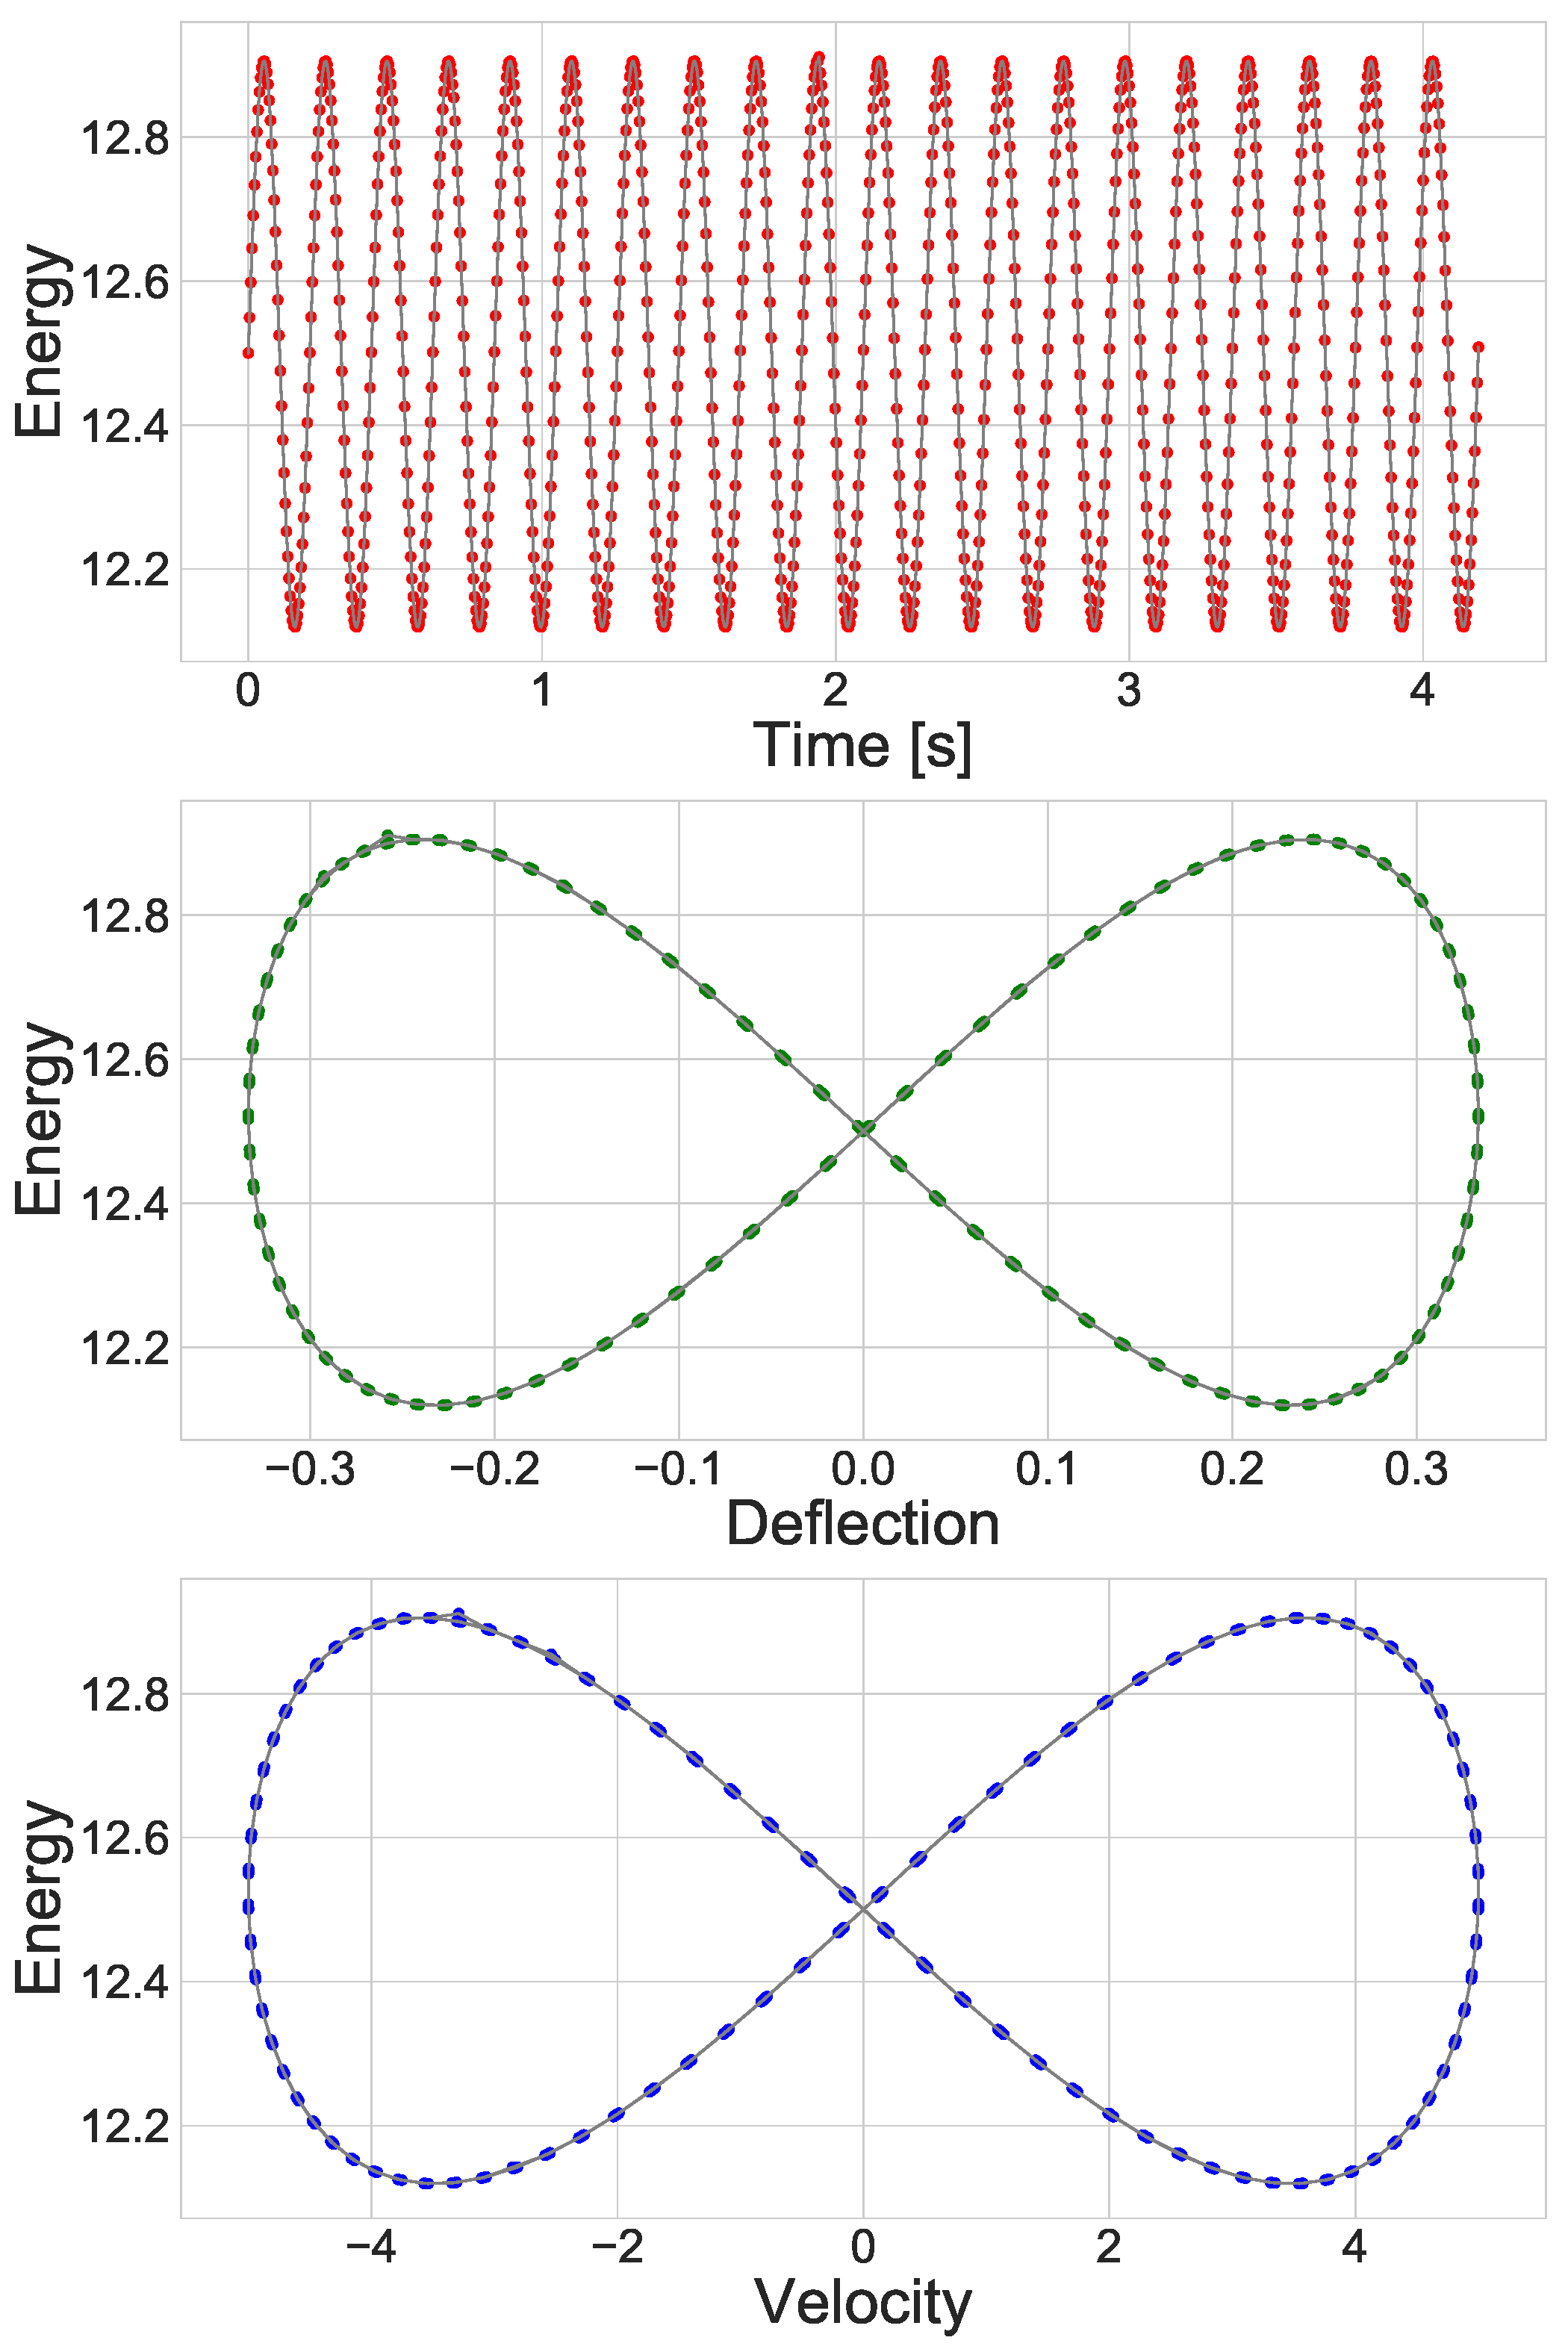
\includegraphics[width=.5\textwidth]{energy_eulercromer.pdf}}
\captionof{figure}{Euler-Cromer módszer\\Fent: Idő - Energia\\Középen: Kitérés - Energia\\Alul: Sebesség - Energia}\label{fig5}

\subsection{Futásidő}
A negyedik és egyben utolsó feladat a program futásidejének vizsgálata volt a szimuláció lépésszámának függvényében. A lépésszámot két módon növelhetjük:

\begin{enumerate}
    \item A periódusok számának növelésével
    \item A periódusonkénti $dt$ lépésköz hosszának csökkentésével
\end{enumerate}
Jelen esetben az egyszerűség kedvéért az első módszer segítségével határoztam meg a futásidő változását. Az egyéb paramétereket a \ref{tab3}. táblázatban szereplőkkel megegyezően vettem fel. Az idő méréséhez a chrono library \code{std::chrono::steady\_clock} \code{std::chrono::microseconds}, mikroszekundum pontosságú függvényét használtam. A szimulációs paraméterek itt is az \ref{tab1}. táblázatban szereplőekkel azonosak voltak, azonban a futásidőket $10$ és $130$ darabszámú periódus közti futtatásokra vizsgáltam. A kapott értékek a \ref{fig6}. ábrán láthatóak.
\hfill \break \hfill \break
{\centering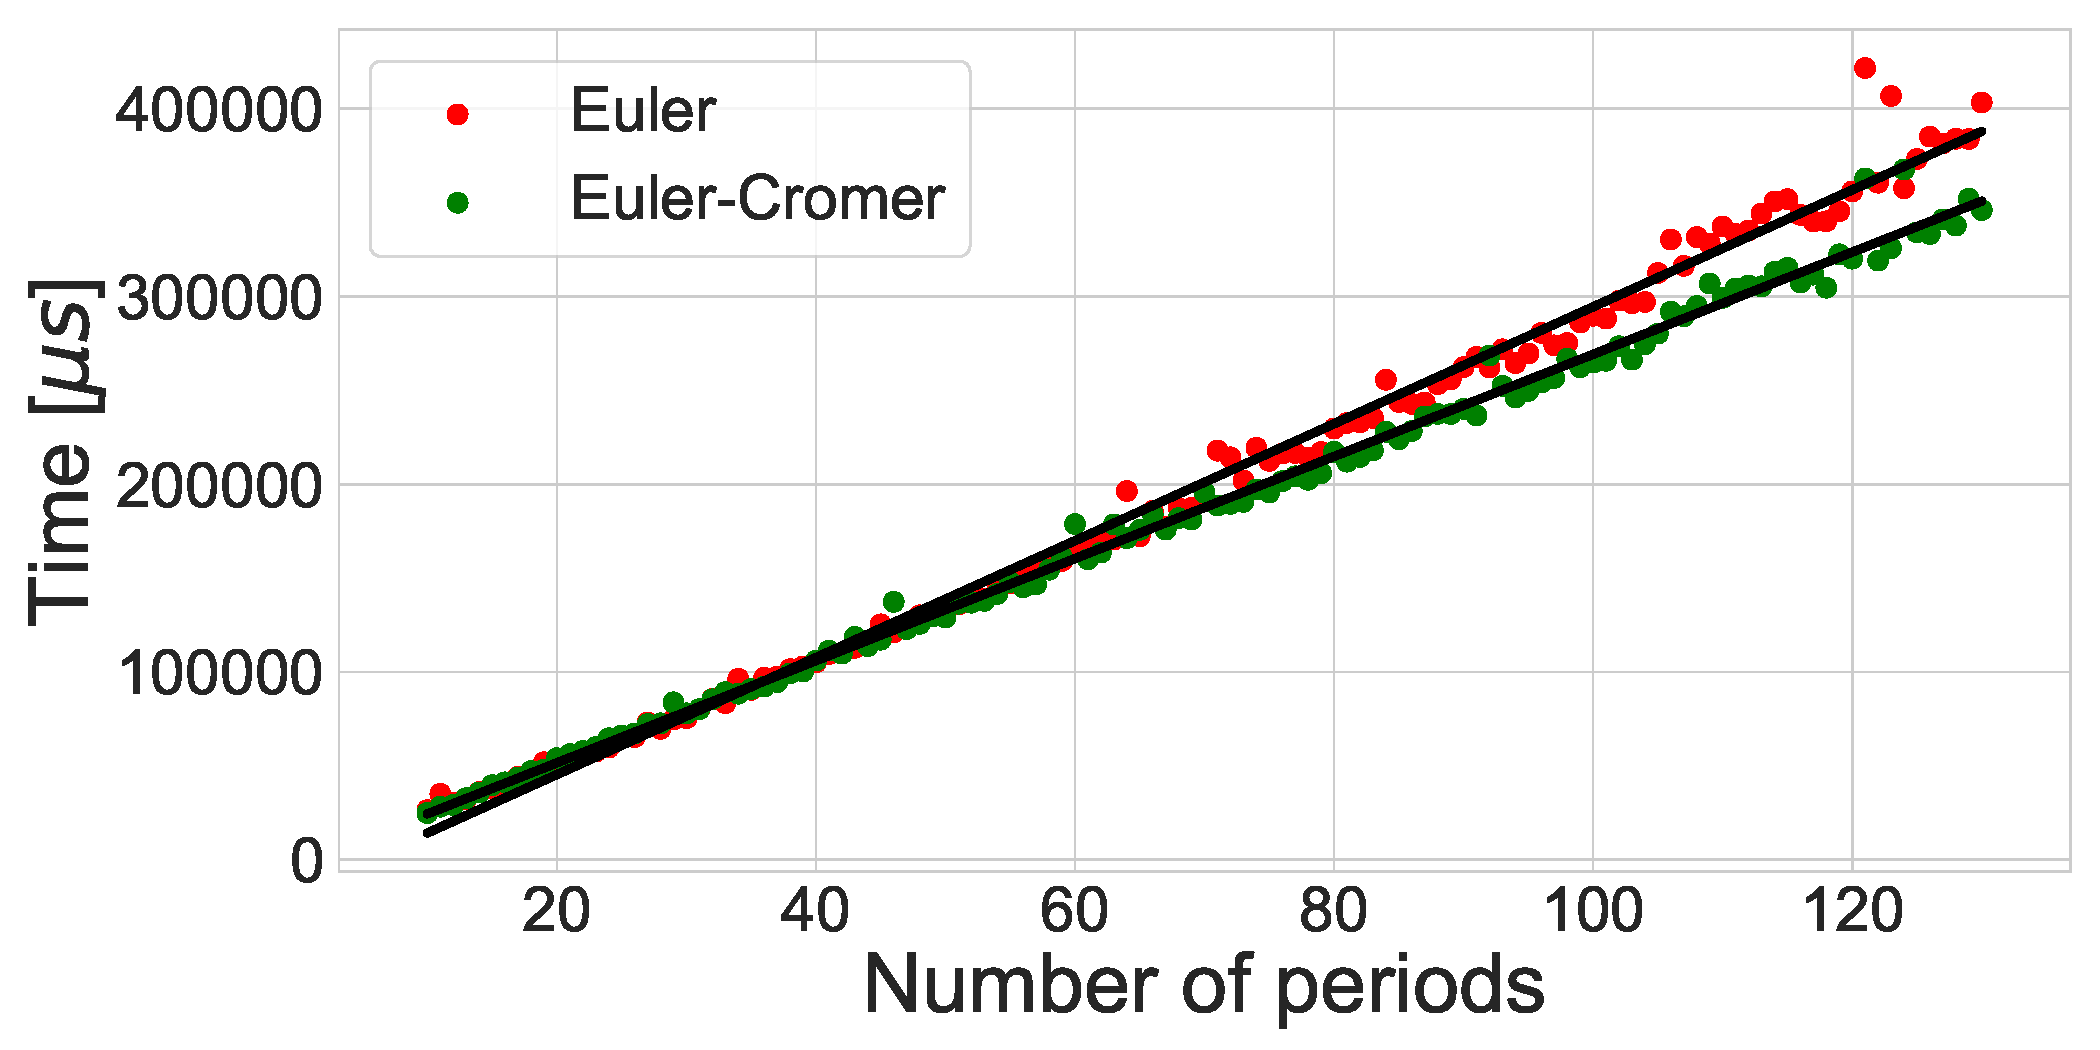
\includegraphics[width=.5\textwidth]{runtime_both.pdf}}
\captionof{figure}{Futásidő\\Fent: Euler módszer\\Alul: Euler-Cromer módszer}\label{fig6}
\hfill \break \hfill \break
Az Euler-Cromer módszer esetében az adatok alapján láthatóan valamivel jobb futásidő érhető el hosszabb távon, azonban ezt a különbséget befolyásolhatták a szimulációt végző számítógépen futó egyéb folyamatok is. \\
Végérvényben biztosra csak azt mondhatjuk, hogy mindkét módszer esetén a periódusok számának növelésével a futásidő lineárisan növekszik. Az Euler módszer esetén a futásidőt az alábbi függvény adja meg a mérések során:

\begin{equation}
    T \left( P \right) = \left( 4493 * P - 1736 \right)\ \mu s
\end{equation}

Míg az Euler-Cromer módszer esetében:

\begin{equation}
    T \left( P \right) = \left( 4097 * P + 15184 \right)\ \mu s
\end{equation}

Ahol $P$ a periódusok darabszámát jelöli.

\section{Diszkusszió}
A Számítógépes szimulációk laboratórium első gyakorlatán kitűzött témához - az 1D harmonikus oszcillátorhoz - tartozó feladatokat kivétel nélkül sikerült a rendelkezésre álló időn belül megoldani. A vele lévő munka során felmerülő akadályokat - mind a \LaTeX, mind a \code{C++} és \code{Jupyter/Python} programozás terén sikerült áthidalni. \\
Az első feladatban kizárólag az Euler-Cromer módszerhez tartozó kitérés-idő és sebesség-idő grafikont csatoltuk, azonban a gyakorlathoz létrehozott GitHub repository-ban\cite{github} található notebookban az Euler módszerhez tartozó is megtalálható. A futásidők vizsgálatánál a két módszer közötti eltérést biztosra nem tudom megmondani, hogy mi okozhatja. Mivel egy elég gyenge laptopon futott azok kiértékelése, ezért lehetséges, hogy valamilyen épp lefutó háttérprogram zavarta meg a kapott adathalmazt. Tisztán látszott azonban, hogy a mindkért esetben lineáris a függés a szimulált periódusok száma és a futásidő között.


\section{Megjegyzések}
A dokumentumban található képek 150 dpi felbontású, \code{.pdf} kiterjesztésű forrásból származnak, amiket a \code{matplotlib} package \code{savefig} függvényének segítségével mentettem le. Ezek miatt a jegyzőkönyv néha lassan tölt be, azonban a már többször említett GitHub repository-ban az nagyon könnyen olvasható. (Ennek az oka feltehetően az, hogy GitHub-on megnyitva az oldal az egész PDF-et betölti, míg egy offline PDF olvasó csak egy adott tartományban levő részeket az optimalizáció miatt.) A további jegyzőkönyvek lehetőleg szintén ezt a formátumot fogják követni. \\
Remélhetőleg az itt elsajátított tudást sikeresen alkalmazhatom majd a további problémák megoldásához is.

\end{multicols}
\hrulefill